\chapter{Scientific Background}
\label{chap:scientific_background}

\section{Active Galactic Nuclei}
\label{sec:agn}

Active Galactic Nuclei (AGN) refers to the central region of active Galaxies. Those objects are among the most luminous objects in the universe, with bolometric luminosities ranging from $10^{41}$ to $10^{48} \ \mathrm{erg \ s^{-1}}$, outshining entire galaxies by several orders of magnitude \parencite{peterson1997introduction}.First explanation tries were unusually dense star clusters or repeated supernova explosions as power sources, but these models soon proved insufficient to account for the observed luminosities, which spans over the entire electromagnetic spectrum. Today it is understood, that these enormous luminosities are powered by accretion of matter onto a supermassive black hole (SMBH) in the center of the AGN. The most common model for this accretion is a hot, rotating accretion disk around the SMBH, which is responsible for most of the observed radiation \parencite{shakura1973black}.\\
The following sections will outline the key components of an AGN, introduce the unification model that connects various AGN types, and summarize common classification schemes. A special focus will be on AGN variability, which plays a central role in the reverberation mapping analysis conducted in this thesis.



\begin{figure}[!ht]
	\centering
	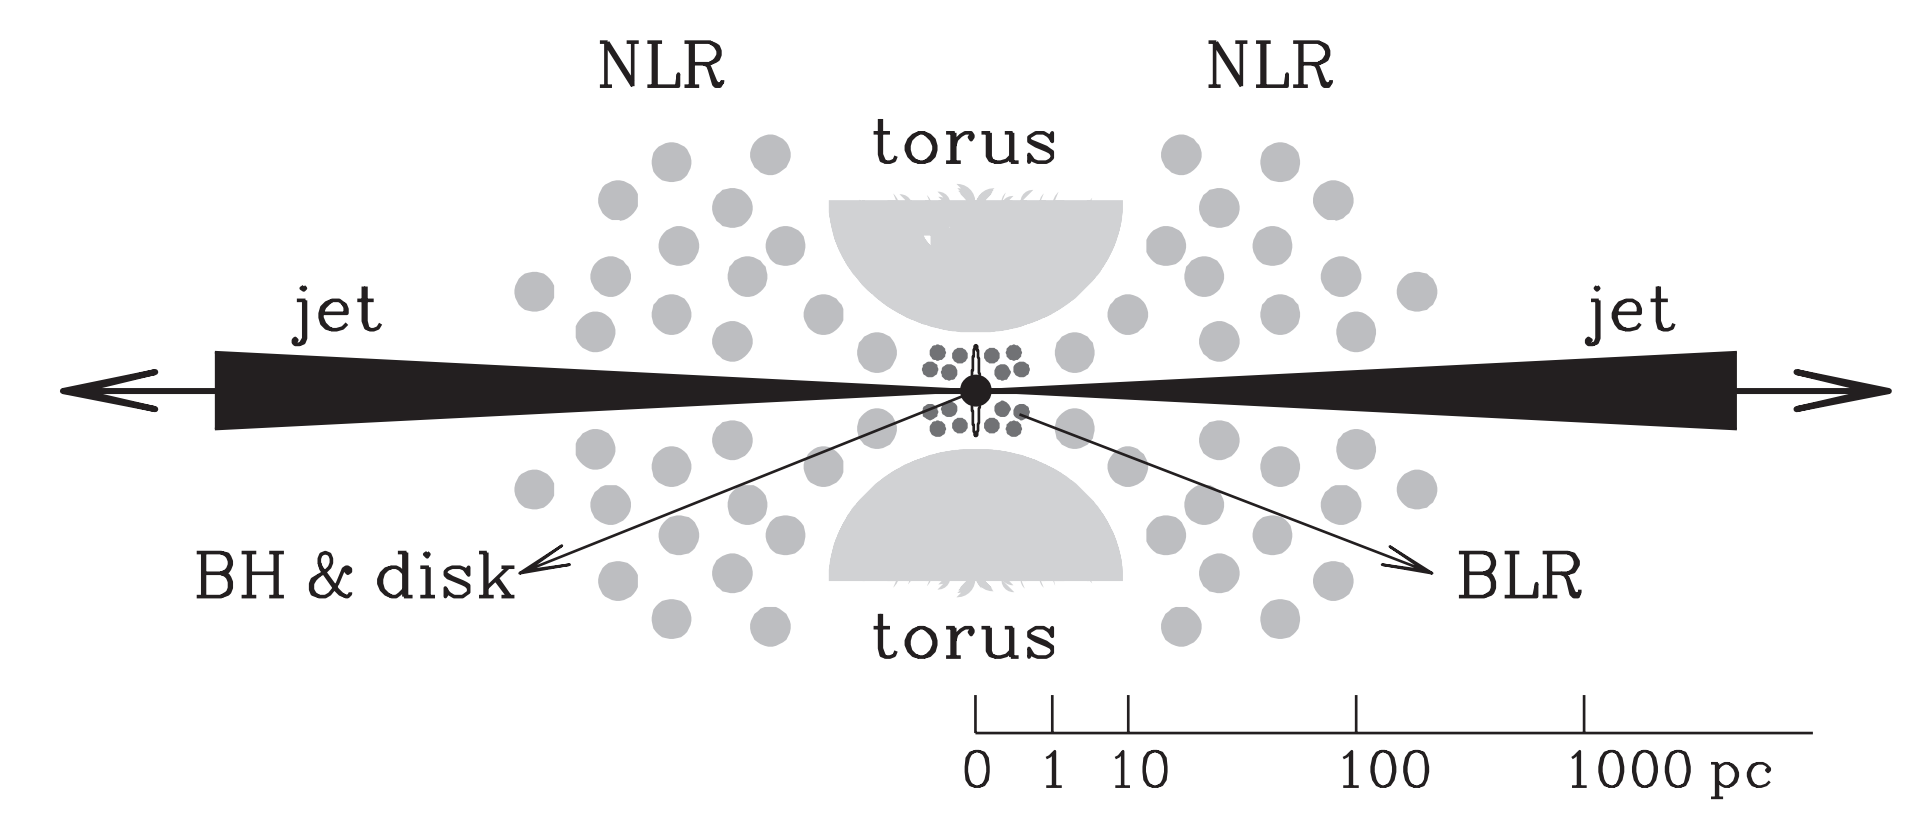
\includegraphics[width=0.75\textwidth]{pictures/Chapter2/AGN_standard_paradigm.png}
	\caption{Different components of an AGN. Adapted from \parencite{mo2010galaxy} Figure 14.3.}
	\label{fig:agn_structure_mo}
\end{figure}


\subsection{Structure and Spectral Features of an AGN}
\label{sec:agn_structure}

Figure \ref{fig:agn_structure_mo} illustrates a schematic structure of an AGN, which can be distributed in multiple components: a central supermassive black hole (SMBH), an accretion disk that feeds the SMBH, a surrounding dusty torus, and ionized gas regions known as the broad-line region (BLR) and narrow-line region (NLR). Additionally the figure shows relativistic jets that launches perpendicular to the accretion disk plain, which will not be further discussed in this section, due to lack of relevance for this thesis.


\subsubsection{Supermassive Black Hole and Accretion Disk}

The center of an AGN is formed by a supermassive black hole (SMBH), with typical masses between $10^6\,M_\odot$ and $10^{10}\,M_\odot$. It does not contribute to the AGN spectrum by itself, but acts as the central engine for all observed spectral features of the AGN. It dominates the gravitational potential and other then inactive Galaxies, like the milky-way, it is surrounded by an accretion disk. Due to viscosity processes within the disk, like turbulent friction or magneto-rotational instability, the angular momentum of the matter is getting transported further out of the disk, which leads to a spiraling matter flow inwards the SMBH. 
The accretion disk itself is a geometrically thin and optically thick structure composed of ionized gas in differential rotation around the SMBH. The disk consists primarily of ionized hydrogen and helium, with traces of heavier elements. It extends from the innermost stable circular orbit (ISCO) near the event horizon out to distances of several light-days. The radial extent of the disk is relatively small compared to  galactic scales and typical ranges from a few light-hours to a few light-days, corresponding to about $10^{-3}$ to $10^{-2}$\,pc \parencite{netzer2013agn,hickox2018obscured, shakura1973black}.  \\
During the accretion process a significant fraction of the gravitational energy of the matter is transformed into thermal radiation, which accounts for the enormous luminosity observed in AGNs and heats the accretion disk up to very high temperatures depending on the size of the SMBH. As an example, the maximum effective temperature for an accretion disk around a SMBH with $M = 10^8,M_\odot$ is on the order of several $\times 10^5$ K, leading to UV and optical emission. In comparison, disks around stellar-mass black holes reach much higher temperatures (up to a few $\times 10^6$ K), emitting mostly in X-rays. Due to the temperature gradient with hotter regions in the inner disk, the emitted spectrum can not be described as a single black-body. Instead, it results from combination of many black-body-like components at different temperatures, often referred to as a multi-color black-body. This creates a broad optical-UV continuum emitting ionized photons, which play a crucial role for the other spectral features. They interact with the surrounding gas clouds near the nucleus, causing photo-ionization followed by recombination. This process leads to different types of strong emission lines, which are characteristic features of AGN spectra \parencite{netzer2013agn, osterbrock1989agn}.


\subsubsection{Broad-Line and Narrow-Line Region}

Geometrical above and below the accretion disk plain, lies a distribution of gas clouds, which are photo-ionized by the energetic photons of the accretion disk continuum. The innermost of these clouds is the broad-line region (BLR), located at distances of a few light-days to light-weeks from the central SMBH (see Figure \ref{fig:agn_structure_mo}). The BLR consists of dense gas clouds with electron densities of $n_e \sim 10^9$–$10^{11} \mathrm{cm^{-3}}$, moving at high velocities of several thousand kilometers per second due to the strong gravitational influence of the SMBH. These velocities lead to a significant Doppler broadening of permitted emission lines and line widths of around $3000\ \mathrm{km \ s^{-1}}$. As described earlier, the BLR is primarily photo-ionized by the continuum radiation emitted from the accretion disk. As a result, the line emission from this region is strongly correlated with the continuum emission, which is particularly important for a reverberation mapping analysis, which will be discussed later in Section \ref{sec:reverberation_mapping}.\\ The exact geometry of the BLR remains uncertain, with models ranging from a spherical distribution of clouds to a flattened disk-like structure. Broad emission lines appear in permitted transitions such as H$\alpha$, H$\beta$ and Ly$\alpha$. \parencite{netzer2013agn, osterbrock1989agn, peterson1997introduction}
\\
Even further out lies the narrow-line region (NLR). The gas in this region moves at much lower velocities, resulting in emission lines with widths typically below $1000\ \mathrm{km \ s^{-1}}$. In contrast to the BLR, the NLR allows both permitted and forbidden transitions. Forbidden lines, such as [O III] $\lambda5007$, arise because collisional de-excitation is inefficient at the relatively low densities of the NLR ($n_e \sim 10^2$–$10^6 \mathrm{cm^{-3}}$) \parencite{osterbrock1989agn}. The narrow [O III] $\lambda5007$ line was used to intercalibrate the spectra of the various observations employed in this thesis (see Chapter \ref{campaign_and_analysis}).




\subsubsection{Dusty Torus}

Surrounding the accretion disk and broad-line region is the dusty torus, a geometrically thick and optically dense structure composed of gas and dust. It extends from a radius, where dust can survive the intense radiation of the accretion disk, out to scales of a few parsecs. The torus likely has a clumpy distribution and plays a crucial role in the unified model of AGNs which will be discussed in a later section \parencite{netzer2013agn,hickox2018obscured}.
The dust in the torus absorbs a significant fraction of the UV and optical radiation emitted by the accretion disk and re-emits it thermally in the infrared. As a result, AGNs typically exhibit strong infrared emission, with the peak wavelength depending on the temperature of the dust in the torus. This reprocessed radiation provides an important observational signature and can be used to trace obscured AGN activity, especially in AGNs where the central region is hidden from direct view \parencite{netzer2013agn}.



\subsection{Classification}
\label{sec:classification}

Next to the classical Hubble classification, AGN get classified in subgroups based on their spectral features, which are strongly dependent to their intrinsic structure. The key parameters for this classification are luminosity, emission-line profiles and radio properties. Based on those parameters AGN get grouped into Seyfert galaxies, quasars and radio galaxies. Seyfert galaxies are further subdivided based on the appearance of broad and narrow emission lines. Seyfert I galaxy spectra show both broad and narrow emission lines, while Seyfert II galaxy spectra show only narrow emission lines. Besides those main classes there are additional sub-classes including narrow-line Seyfert I galaxies (NLS1s), low-ionization nuclear emission-line regions (LINERs), and jet-dominated sources such as BL Lac objects or blazars \parencite{antonucci1993unified, urry1995unified}. 


\begin{figure}[!ht]
	\centering
	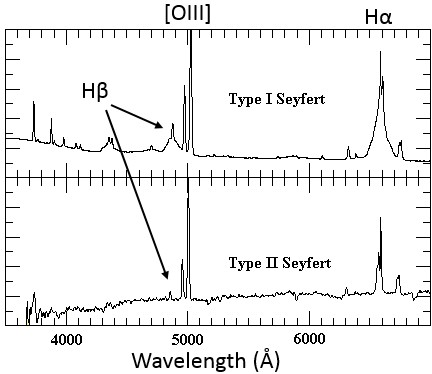
\includegraphics[width=0.75\textwidth]{pictures/Chapter2/Syefert1vsSeyfer2}
	\caption{An example of Seyfert I and Seyfert II spectra illustrating their differences. Broad lines, such as the highlighted $H\alpha$ and $H\beta$, are only present in the Seyfert I spectrum, whereas forbidden [O III] lines are visible in both cases. Adapted from \parencite{researchgate_seyfert2025}.}
	
	\label{fig:Seyfert1vsSeyfert2}
\end{figure}



\subsubsection{Seyfert Galaxies}

Seyfert galaxies are named after Carl K. Seyfert, who in 1943 observed spiral galaxies characterized by exceptionally bright nuclei and strong emission lines in their optical spectra \parencite{seyfert1943nuclear}. They a classified mainly the sub-classes Seyfert I and Seyfert II based on the presents of broad emission lines. Figur \ref{fig:Seyfert1vsSeyfert2} highlights the differences of the spectra of Type I and Type II Seyfert galaxies.\\
Seyfert I galaxies, like NGC 4593, show both broad and narrow emission lines in their optical spectra. The broad lines, such as $H_\alpha$ and $H_\beta$, have a full width at half maximum (FWHM) of typically several thousand kilometers per second and arise from the high-velocity BLR. In contrast, narrow lines, including prominent forbidden transitions like [O\,\textsc{iii}] $\lambda5007$ or [N\,\textsc{ii}] $\lambda6584$, originate from the lower-velocity NLR \parencite{osterbrock1989agn, peterson1997introduction}. The presence of both components in the spectrum allows for a clear classification as a Seyfert 1 galaxy, which is the case for NGC4593. More to NGC4593 in section \ref{NGC4593}.\\
In comparison, Seyfert II galaxies lack these broad components in their optical spectra, likely due to orientation-dependent obscuration by the dusty torus. So the classification of a Seyfert galaxies strongly depends on the viewing angle of the observer, which is the key point for the Unified Model of AGN, which will deepened in section \ref{sec:unification_model}.\\ Another notable subclass are the so-called narrow-line Seyfert 1 galaxies (NLS1s). Despite their classification as Seyfert 1, the broad permitted lines in their spectra exhibit unusually small widths, with FWHM $<$ 2000 km\,s$^{-1}$. They often show strong Fe\,\textsc{ii} emission complexes and steep soft X-ray spectra. NLS1s are thought to have low-mass black holes accreting at high Eddington rates, suggesting they may represent a young evolutionary phase of AGN activity \parencite{osterbrock1985nls1, netzer2013agn}.



\subsubsection{Others}

Next to Seyfert galaxies, there are several other classes of AGN. Quasars, which stands for quasi-stellar radio sources, are even more luminous than Seyfert galaxies and are typically found at higher redshifts. While the host galaxies of Seyfert galaxies are still observable, quasars completely outshine their host galaxies. Since quasars show similar emission characteristics to Seyfert galaxies, the modern distinction is based mainly on luminosity: quasars are classified as high-luminosity AGNs, while Seyfert galaxies represent the lower-luminosity end \parencite{netzer2013agn}.\\
Radio galaxies are defining another AGN class. There are characterized by their strong radio emission and prominent jets, often associated with elliptical host galaxies. When their jets are aligned close to our line of sight, they are observed as blazars or BL Lac objects, which exhibit rapid variability and featureless optical spectra due to relativistic beaming \parencite{netzer2013agn}.\\
Finally, LINERs are low-luminosity AGNs with spectra dominated by low-ionization emission lines. The physical origin of their ionization mechanism is still debated, and in some cases, they may not be powered by accretion at all \parencite{netzer2013agn}.\\\\
While these classifications are based primarily on spectral characteristics, many of the observed differences between AGN types can be attributed to orientation effects. The Unified Model of AGN provides a framework that explains this apparent diversity through a common internal structure, viewed from different angles.

\subsection{Unification Model}
\label{sec:unification_model}

Figure \ref{fig:agn_sed} shows an illustration of the Unification Model, which was postulated by Robert Antonucci in 1993. He proposed that the visible differences in AGN spectra are not due to fundamentally different structures. Instead, they arise mainly from the viewing angle toward the AGN center and from obscuration by the dusty torus \parencite{antonucci1993unified}.\\
The figure shows with what type the same AGN would get classified depending on the observers viewing angle. Like mentioned before, the dusty torus plays a key role here, as it surrounds the central region of the AGN, the accretion disk and the fast-moving BLR. If the observer's line of sight is blocked by the torus, only radio emission and narrow-line emission from the NLR outside the torus can be detected. In this case, the AGN appears as a Seyfert 2 galaxy, since the broad emission lines from the BLR and the optical/UV radiation from the accretion disk are obscured. The observer essentially views the AGN from a flat angle, looking directly at the torus.\\
If, on the other hand, the observer has a direct view into the central region of the AGN, not obscured by the torus, the fast moving gas clouds of the BLR as well as the optical/UV emission continuum from the accretion disk become visible. So both, broad and narrow emission lines, can be observed, which classifies it as a Seyfert 1 Galaxy \parencite{antonucci1993unified}.\\
The same principle applies to other AGN classes. Quasars can be considered the high-luminosity counterparts of Seyfert galaxies, where orientation and torus obscuration likewise affect their observed properties. Blazars, on the other hand, are seen when the relativistic jet is aligned closely with the observer’s line of sight, leading to strong Doppler boosting, which makes the radiation appear significantly brighter and shifted to higher frequencies than it intrinsically is \parencite{urry1995unified}.\\
Although the classical Unification Model treats AGN classification as fixed and purely geometry-driven, some AGNs have been observed to change their spectral type over time. These so-called "changing-look AGNs" demonstrate that a purely orientation-based interpretation, such as the Unification Model, cannot explain all observed phenomena. They suggest that intrinsic changes, such as variations in accretion rate or obscuring material, can also affect the classification \parencite{ricci2022changinglook}.




\begin{figure}[!ht]
	\centering
	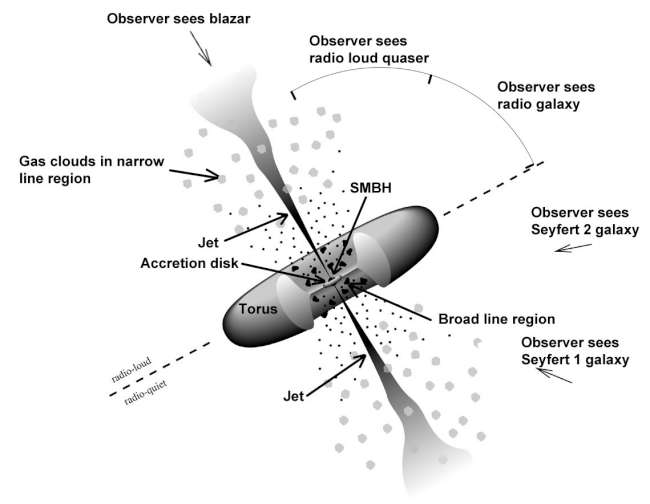
\includegraphics[width=0.9\textwidth]{pictures/Chapter2/AGN_unified_model.jpg}
	\caption{Unification model of an AGN \parencite{fermi2025figure1}.}
	\label{fig:agn_sed}
\end{figure}



\subsection{Variability}
\label{sec:variability}

Apart from changing-look AGNs that change their classification, many AGNs show significant and continuous variation in their emitted spectra. Unlike the much longer time period of changing-look AGNs, this variability can be observed over timescales of hours, days up to years across all the electromagnetic spectrum, with different fluctuation velocities. Averagely Higher-energy emission, like X-rays, shows faster and stronger variations than optical or infrared emission, which makes them energy-dependent. These timescales range from hours, to days and to years, showing generally a stochastic nature \parencite{Ulrich1997}.\\ 
A way to explain the variability of an AGN are instabilities in the spiraling accretion flow onto the SMBH. Processes like magnetic turbulence in the corona, local fluctuations in the accretion rate or thermal inhomogenities within the disk could influence the continues accretion flow, creating fluctuation within the emitting regions. The energy-dependence can be understood considering the regions where the radiation originates from. High-energy emission arises from the innermost part of the accretion flow, mainly from the corona of the SMBH. It is a very compact region and the emitting volume is much smaller compared to the regions responsible for lower-energy emission, which are located at much larger radii. Following that, the light-crossing timescale $t_lc = R/c$, which defines how long light takes to pass the region, is much shorter for the compact high energy volume. In contrast to that, regions with larger radii, like the optical or infrared emitting regions, have much longer light-crossing timescale , resulting in correspondingly slower variability \parencite{Ulrich1997, McHardy2006}.\\
Because of the variations being noticeable in small timescales, like hours ore days, it can be utilized to get more information about the size and the structure of emitting regions with an reverberation mapping analysis, which will be discussed in the next section.



\section{Reverberation Mapping}
\label{sec:reverberation_mapping}

The main focus of this work is a classic reverberation mapping analysis of the Broad Lines of NGC 4593. This observational technique allows to probe the structure of the BLR around the SMBH inside the AGN. This technique bases on the time delay or time lag between the continuum's variation and the correlated response of the broad lines. With this calculable time lag it is possible to assume the geometry of the BLR and calculating the mass of the SMBH.  


\subsection{Principle}
\label{subsec:rm_principle}

The fundamental assumption in reverberation mapping is that fluctuations in the observed continuum luminosity drive corresponds to the fluctuations in the emission-line flux, with a measurable time delay. Like mentioned earlier, continuum fluctuations from the accretion disk serve as the ionizing source, illuminating the surrounding BLR. With variation in the continuum luminosity, the emission-line response follows these continuum variations with a measurable time lag \parencite{Cackett2021}.
This time lag $\tau$ is corresponding to the average light-travel distance from the photoionization continuum to the line emitting regions. Furthermore it is possible to approximate the characteristic radius of the BLR depending on $\tau$ following this approximation: $R_{\mathrm{BLR}} \approx c \cdot \tau$. With different time lags from emission lines origination from different regions it is possible to infer the geometry of the BLR. A BLR with a thin shell of clouds would produce a more uniform lag, whereas a broad distribution of clouds produces a range of lags. In principle, reverberation mapping can be used to 'map' the BLR’s structure by inverting the delays \parencite{peterson1997introduction}.
The response of the BLR's lines is typically assumed as linearly related tho the photo-ionization continuum, leading to the convolution expression:
\\
\begin{equation}
	L\left(t\right) = \int \Psi\left(\tau\right)C\left(t-\tau\right) d\tau
\end{equation}
\\
where $\Psi\left(\tau\right)$ is the transfer function, delivering the BLR's geometric and kinematic information \parencite{horne2004observational}.
While in theory the response of the BLR can be fully described by the transfer function $\Psi\left(\tau\right)$, this thesis focuses on measuring the time lag between continuum and line variations. This lag can be estimated using cross-correlation techniques, which are discussed in the following section.


\subsection{Cross-Correlation Function and Lag Measurement}
\label{subsec:rm_ccf}

In practice, recovering the full transfer function $\Psi\left(\tau\right)$ would require very well-sampled and high signal-to-noise light curves over a duration much longer than the expected lag. Since real monitoring campaigns are often affected by observational gaps and noise, such reconstructions are rarely possible \parencite{horne2004observational,peterson1993}. For this reason, this thesis concentrates on measuring the mean time lag between continuum and emission-line variations using the Interpolated Cross-Correlation Function (ICCF) method.\\
Measuring the same objects over a span of time, it is possible to determine the correlation coefficient (CCF)  as a function of the time shift $\tau$ between two light curves, e.g. the variable light curve of the ionizing continuum and the light curve of a broad emission line. By sliding one curve relative to the other, the ICCF quantifies how well the variations match for each lag.  In this context, two types of lags are defined: the lag corresponding to the maximum correlation $\tau_{\mathrm{peak}}$ and the centroid lag $\tau_{\mathrm{centroid}}$. $\tau_{\mathrm{centroid}}$ gets calculated over all points of the CCF, that are above a selected threshold which is typically $80\%$ of the CCF. Since the centroid lag is generally considered a more robust representation of the mean light-travel time of the BLR \parencite{peterson2004}, it is used in this thesis.\\
The uncertainty of the measured lag is estimated using a Monte Carlo approach combining Flux Randomization (FR) and Random Subset Selection (RSS) \parencite{peterson1998,peterson2004}. In the FR step, each flux value is randomly perturbed according to its measurement uncertainty. In the RSS step, a subset of the data points is drawn at random with replacement, preserving the original sample size. For each realization, the ICCF analysis is repeated, resulting in a distribution of centroid lags. The median of this distribution is adopted as the final lag measurement, while the 16th and 84th percentiles are taken as the $1 \sigma$ confidence interval, accounting for both measurement noise and the effects of uneven temporal sampling.


\subsection{Black-Hole Mass}
\label{subsec:rm_bh_mass}

With the measured rest-frame centroid lag $\tau_{\mathrm{centroid}}$ from the ICCF analysis and the velocity width of the broad emission line, the mass of the central supermassive black hole (SMBH) can be estimated under the assumption that the BLR gas is gravitationally bound and its motions are dominated by the SMBH potential \parencite{peterson2004}. The distance to the BLR is given by

\begin{equation}
	R_{\mathrm{BLR}} = c \cdot \tau_{\mathrm{centroid}}
\end{equation}
and, combined with the line-of-sight velocity dispersion $\Delta V$ of the BLR gas, the virial product is defined as:

\begin{equation}
	M_{\mathrm{vir}} = \frac{R_{\mathrm{BLR}}\,\Delta V^2}{G}.
\end{equation}
The physical black hole mass is then obtained by applying a scale factor $f$, which accounts for the unknown geometry, kinematics, and inclination of the BLR:
\begin{equation}
	M_{\mathrm{BH}} = f \cdot M_{\mathrm{vir}}.
\end{equation}
Following \textcite{onken2004}, a mean value of $f$ is adopted, calibrated by aligning reverberation-based masses with the $M_{\mathrm{BH}}-\sigma_*$ relation observed in not-active galaxies. Here, $\sigma_*$ describes the stellar velocity dispersion of the galactic bulge. The actual scale factor can still vary between individual AGN because of differences in their geometry and orientation, which results in systematic uncertainties in the SMBH mass estimation. Still, the calibration of $f$ against $M_{\mathrm{BH}}-\sigma_*$ delivers a well-established methode for estimation the SMBH mass and will be used in this thesis.



\section{Bowen Fluorescence}
\label{sec:bowen_fluorescence}

The mechanism known as Bowen Fluorescence was first described by I.S. Bowen in 1934 to explain unexpected emission lines in nebular spectra \parencite{bowen1934}. It is a multi-stage process called resonant line pumping. I this process Photons, emitted by an ion, hits randomly another ion of a different species with a matching permitted transition, and excites it via absorption due to a near-wavelength coincidence. The resulting de-excitation leads to enhanced emission lines that would otherwise be too weak to detect through normal recombination or collisional excitation. In AGN, Bowen Fluorescence typically involves He\textsc{ii} Lyman-$\alpha$ photons at 303.78\AA, which excite O\textsc{iii} ions and, in a secondary step, N\textsc{iii} ions. The result is the emission of characteristic ultraviolet and optical lines with similar correlation \parencite{selvelli2007, baldini2023}.\\
Similar fluorescence processes are also known for other ions. In this thesis, particular focus is placed on the O\textsc{i}$\lambda$8446 emission line. Its strength cannot be explained by recombination processes alone and is commonly attributed to Ly$\beta$ fluorescence. In this process, hydrogen Ly$\beta$ photons at 1025.72\AA are absorbed by neutral oxygen due to a near-resonant transition. This enhances the O\textsc{i} emission through a separate, but related, fluorescence mechanism \parencite{grandi1980}.\\
Although Ly$\beta$-pumped O\textsc{i}$\lambda$8446 emission is independent of the classical Bowen mechanism, both processes share the fundamental principle of resonant line pumping, where photons from one species excite another species. As a result, both mechanisms provide valuable diagnostic information about the physical conditions and radiation field in AGN broad-line regions \parencite{grandi1980, selvelli2007}. In this work, the O\textsc{i}$\lambda$8446 emission line is investigated in the context of possible fluorescence excitation in NGC 4593.





